\documentclass[conference]{IEEEtran}
\IEEEoverridecommandlockouts
% The preceding line is only needed to identify funding in the first footnote. If that is unneeded, please comment it out.
\usepackage{cite}
\usepackage{amsmath,amssymb,amsfonts}
\usepackage{algorithmic}
\usepackage{graphicx}
\usepackage{textcomp}
\usepackage{xcolor}
\usepackage{booktabs}
\usepackage{hyperref}
\usepackage{url}
\def\BibTeX{{\rm B\kern-.05em{\sc i\kern-.025em b}\kern-.08em
    T\kern-.1667em\lower.7ex\hbox{E}\kern-.125emX}}

\begin{document}

\title{Trinity: A Neuro-Symbolic Multi-Agent Framework for Stateful Network Penetration Testing}

\author{%
\begin{minipage}[t]{0.30\textwidth}
\centering
\textbf{S M Udhaya Sankar}\\
\textit{Professor}\\
Dept of CSE (Cyber Security)\\
R.M.K. College of Engineering\\
and Technology, Thiruvallur, India\\
{\small udhaya3@gmail.com}

\vspace{0.4cm}

\textbf{Jayachandran J A}\\
\textit{Student}\\
Dept of CSE (Cyber Security)\\
R.M.K. College of Engineering\\
and Technology, Thiruvallur, India\\
{\small jayacy023@rmkcet.ac.in}
\end{minipage}%
\hfill
\begin{minipage}[t]{0.30\textwidth}
\centering
\textbf{Dharini N}\\
\textit{Associate Professor}\\
Dept of CSE (Cyber Security)\\
R.M.K. College of Engineering\\
and Technology, Thiruvallur, India\\
{\small dharinics@rmkcet.ac.in}
\end{minipage}%
\hfill
\begin{minipage}[t]{0.30\textwidth}
\centering
\textbf{Jaisurya S}\\
\textit{Student}\\
Dept of CSE (Cyber Security)\\
R.M.K. College of Engineering\\
and Technology, Thiruvallur, India\\
{\small jaiscy022@rmkcet.ac.in}

\vspace{0.4cm}

\textbf{Prasanth C M}\\
\textit{Student}\\
Dept of CSE (Cyber Security)\\
R.M.K. College of Engineering\\
and Technology, Thiruvallur, India\\
{\small cmprcy012@rmkcet.ac.in}
\end{minipage}%
}

\maketitle

\begin{abstract}
Penetration testing remains both critical and labour-intensive in modern cybersecurity practice. Current automated approaches built on monolithic large language models (LLMs) struggle with statelessness, tend to hallucinate dangerous commands, and cannot reason over multi-hop attack paths that span multiple hosts and services. We present \textbf{Trinity}, a neuro-symbolic, multi-agent framework for stateful network penetration testing that tackles these limitations through three key innovations. Our \textit{Neuro-Symbolic Safety Loop} enforces deterministic Pydantic-based validation on every generated attack command, blocking out-of-scope or denial-of-service operations before they can execute. Alongside this, \textit{Graph-Based Knowledge Hygiene} maintains a Neo4j attack-path graph modelling verified relationships between hosts, open ports, and associated CVEs---ensuring the agent reasons only over empirically confirmed network facts. The framework also incorporates a \textit{Self-Healing Execution} mechanism that detects tool-level failures (e.g., Nmap syntax errors, Metasploit connection timeouts) and regenerates corrected commands through an LLM feedback loop governed by a circuit-breaker pattern. LangGraph orchestrates the agent as a stateful graph, with real-time vulnerability context drawn from a ChromaDB vector store populated by live NVD feeds. In controlled multi-host lab scenarios, Trinity improved reconnaissance completeness and command reliability over stateless LLM baselines while upholding strict scope and safety compliance. This work establishes a reproducible, safety-conscious benchmark for autonomous network penetration testing agents.
\end{abstract}

\begin{IEEEkeywords}
Penetration Testing, Multi-Agent Systems, Large Language Models, LangGraph, Graph-Based Knowledge Hygiene, Neuro-Symbolic AI, Self-Healing Execution, Network Security Automation.
\end{IEEEkeywords}

% ─────────────────────────────────────────────────────────────────────────────
\section{Introduction}
% ─────────────────────────────────────────────────────────────────────────────

As networked infrastructure grows more complex, manual penetration testing has become increasingly time-consuming and difficult to scale. Consider that a single enterprise network might expose hundreds of hosts across multiple subnets, each running services with vulnerability profiles that shift whenever patches roll out or new CVEs surface. Security professionals face the demanding task of tracking reconnaissance findings, mapping lateral movement opportunities, staying within scope, and avoiding detection---a cognitive burden that makes human-conducted engagements both expensive and inherently inconsistent.

The rise of large language models (LLMs) has naturally sparked interest in automating security workflows. Early work showed that general-purpose LLMs could handle rudimentary reconnaissance and suggest exploitation strategies \cite{happe2023pwnd}. Building on this, later research demonstrated that purpose-built agents could autonomously compromise web applications \cite{fang2024hack}, while locally fine-tuned models proved capable of outperforming commercial alternatives in controlled game environments \cite{rigaki2024hackphyr}. These are encouraging results, but translating them to realistic \textit{network-layer} penetration testing reveals three fundamental gaps.

\textbf{Gap 1 --- Statelessness.} Most LLM-based agents treat each tool invocation in isolation, effectively discarding findings from previous steps. Real penetration testing, however, is fundamentally stateful: learning that Host~A exposes SMB on port~445 only becomes actionable once you have credentials recovered earlier from Host~B. Without persistent, structured memory, agents end up repeating scans, losing intermediate findings, and failing to plan coherent multi-hop attack paths.

\textbf{Gap 2 --- Unguarded Execution.} LLMs sometimes hallucinate tool flags or generate commands that stray outside engagement scope---for instance, including \texttt{-T5} aggressive timing flags that risk network disruption, or targeting addresses beyond the approved subnet. Existing multi-agent frameworks like PentestAgent \cite{shen2024pentestagent} and BreachSeek \cite{breachseek2024} rely on prompt-level instructions to enforce constraints, an approach that breaks down easily under adversarial prompting or model drift.

\textbf{Gap 3 --- Brittle Execution Pipelines.} Network tools fail often---transient connectivity issues, incorrect flag syntax, target-side defences. Current agents tend to either abort on failure or retry blindly, wasting time and generating noisy behaviour. A production-grade agent needs to parse error messages, reason about their cause, and autonomously generate a corrected command within a bounded retry budget.

This paper introduces \textbf{Trinity}, a multi-agent penetration testing framework designed to address these gaps. Our contributions are as follows:

\begin{itemize}
    \item A \textbf{stateful LangGraph orchestration layer} that models the penetration-testing workflow as a directed cyclic graph of specialised agents (Planner, Guard, Executor, Observer), allowing backtracking and context-aware replanning whenever a network path reaches a dead end.
    
    \item A \textbf{Neuro-Symbolic Safety Loop} that intercepts every candidate attack command and validates it against a Pydantic schema encoding scope rules, allowed flag sets, and protocol constraints---before any subprocess gets spawned.
    
    \item A \textbf{Neo4j-backed Attack Graph} storing only verified \mbox{Host $\rightarrow$ Port $\rightarrow$ CVE} triples, giving the Planner a hygiene-enforced knowledge base that grows monotonically as reconnaissance succeeds.
    
    \item A \textbf{Self-Healing Execution} module that parses stderr from Nmap, Metasploit, and Impacket, passes structured error context to an LLM correction agent, and commits a regenerated command---aborting after a configurable circuit-breaker threshold to prevent infinite retry loops.
\end{itemize}

The paper proceeds as follows. Section~\ref{sec:litreview} reviews related work spanning LLM-based pentesting, multi-agent security systems, and knowledge-graph-enhanced reasoning. Section~\ref{sec:methodology} details Trinity's architecture and its four specialist agents. Section~\ref{sec:results} presents experimental results from a controlled CTF environment. Section~\ref{sec:future} discusses limitations and future directions, and Section~\ref{sec:conclusion} concludes.

% ─────────────────────────────────────────────────────────────────────────────
\section{Literature Review}
\label{sec:litreview}
% ─────────────────────────────────────────────────────────────────────────────

Research on automated penetration testing has moved quickly since capable LLMs became widely available. The following survey groups existing work into three thematic clusters: (i)~LLM-driven exploitation agents, (ii)~multi-agent and reinforcement-learning frameworks, and (iii)~knowledge-graph-enhanced security reasoning.

\subsection{LLM-Driven Exploitation Agents}

Happe and Cito \cite{happe2023pwnd} were among the first to show a closed-loop LLM agent performing autonomous vulnerability hunting. Their GPT-based model, given access to shell tools, could conduct reconnaissance and suggest exploits with minimal human guidance. Although the work proved that LLM-driven pentesting was feasible, their agent lacked persistent state---it could not build on prior findings across sessions or chain discoveries into multi-hop attack paths. The authors also flagged privacy concerns around transmitting live network data to cloud-hosted models, a problem they left unresolved.

Fang et al. \cite{fang2024hack} pushed this line of research to the web application layer, building an agent that autonomously exploited real-world web vulnerabilities with a 73\% success rate using GPT-4. The agent's tool orchestration---calling browser automation, SQL injection payloads, and web scrapers in sequence---is impressive, yet its scope stays strictly within the HTTP/HTTPS layer. Network-layer services like SMB, RDP, and SSH, along with the lateral movement patterns linking web compromises to internal hosts, lie outside the model's reach, leaving the most consequential phase of a real intrusion unaddressed.

Rigaki et al. \cite{rigaki2024hackphyr} prioritised privacy by fine-tuning a local 7B-parameter model (Hackphyr) on a synthetic network security game, achieving a 94\% win rate on single-GPU hardware. Running locally sidesteps the cloud data-exfiltration problem, but the training environment is entirely synthetic. The agent has not been tested against multi-stage, real-tool attack chains, so questions remain about how well it would generalise to production networks.

\subsection{Multi-Agent and Reinforcement-Learning Frameworks}

Shen et al. \cite{shen2024pentestagent} introduced PentestAgent, which breaks the pentesting workflow into specialised LLM agents augmented with retrieval-augmented generation (RAG) for surfacing relevant CVE and exploit documentation. Their framework cuts down manual labour in information gathering and report generation considerably. That said, coordination overhead between agents---especially when they must share and reconcile conflicting findings---introduces latency and consistency problems. The authors themselves note that the framework lacks mechanisms for enforcing business-logic constraints during execution.

BreachSeek \cite{breachseek2024} showed a multi-agent system obtaining root-level access on Metasploitable targets through coordinated agent actions. A scanning agent, an exploitation agent, and a reporting agent communicate via message passing, and the system produces human-readable attack narratives. Despite these strengths, the evaluation is largely qualitative. Without standardised benchmarks or statistical comparison against baselines, reproducibility and generalisation are difficult to assess.

Chen et al. \cite{chen2023gailpt} brought Generative Adversarial Imitation Learning (GAIL) to penetration testing, training an agent to mimic expert attack strategies. Imitation learning cuts the exploration cost typical of reinforcement learning and yields agents exhibiting expert-like behaviour in constrained network game environments. The main drawback is heavy dependence on the quality and coverage of the expert knowledge base; attack vectors absent from the training demonstrations are unlikely to be discovered at test time.

Skandylas and Asplunda \cite{skandylas2024autopentest} formalised penetration testing as a Monitor--Analyse--Plan--Execute (MAPE) control loop and demonstrated automated black-box exploitation with a structured tool orchestration layer. The formalisation itself is a valuable conceptual contribution, though the implemented system follows a static methodology that does not adapt based on accumulated contextual evidence, limiting effectiveness against non-standard or partially patched targets.

Security Researchers \cite{rl2024pentest} systematically evaluated reinforcement learning algorithms---Q-learning, DQN, and A3C---for autonomous pentesting, showing that RL agents generalise well across varied network configurations and consistently identify exploitable paths. All experiments, however, ran in simulation; the absence of real-tool integration (Nmap, Metasploit) means these agents have never confronted the non-deterministic failures and noisy outputs characteristic of live network tooling.

\subsection{Knowledge-Graph-Enhanced Security Reasoning}

The CyKG-RAG system \cite{cykgrag2025} augments LLM inference with a cybersecurity-specific knowledge graph, feeding structured threat intelligence into the retrieval context. The approach achieves accurate threat detection and dynamically adapts to newly disclosed vulnerabilities. Its focus, though, is squarely on \textit{detection} rather than \textit{exploitation}: the system spots indicators of compromise but does not plan or execute attack sequences. That detection-only focus is precisely the gap Trinity is designed to fill.

Cyber Attack Analysis Team \cite{kgcyber2024} showed knowledge graph reasoning for cyber attack detection by integrating ATT\&CK framework mappings into a graph model, achieving a 96.8\% detection rate. Their representational approach---encoding hosts, services, and techniques as typed graph nodes---directly informs Trinity's Neo4j attack-path model. Even so, the system's reasoning stops at detection and forensic attribution; it does not generate or validate executable exploit commands.

Most recently, the Penligent AI team \cite{penligent2025} released a professional-grade AI-powered pentesting agent featuring end-to-end automation, multi-agent specialisation, a knowledge-graph-backed CVE database, and natural language interaction for CI/CD pipeline integration. The system sits at the current commercial state-of-the-art and shares architectural ambitions with Trinity. Its stateful context model, however, is proprietary and undocumented, business logic flaw detection has not been independently benchmarked, and the closed-source codebase rules out academic reproducibility. Trinity addresses this gap with a fully open, reproducible implementation and explicit safety constraints validated at the command level.

\subsection{Summary and Positioning}

Taken together, the reviewed work shows that LLMs can contribute meaningfully to penetration testing automation, yet no prior system simultaneously tackles stateful multi-hop reasoning, deterministic safety enforcement, and self-healing execution recovery within a reproducible, open framework. Trinity fills this gap by unifying all three dimensions inside a coherent LangGraph-orchestrated architecture, as detailed next.

% ─────────────────────────────────────────────────────────────────────────────
\section{Methodology}
\label{sec:methodology}
% ─────────────────────────────────────────────────────────────────────────────

\subsection{System Architecture Overview}

We structured Trinity across three logical layers, as shown in Fig.~\ref{fig:arch}: a \textit{Presentation Layer} exposing operator-facing interfaces, an \textit{Application Layer} hosting all intelligent agents and execution engines, and a \textit{Data and Infrastructure Layer} comprising persistent graph and vector stores. Separating concerns this way keeps agent logic, safety enforcement, and data persistence independently testable and replaceable.

\begin{figure}[h]
\centering
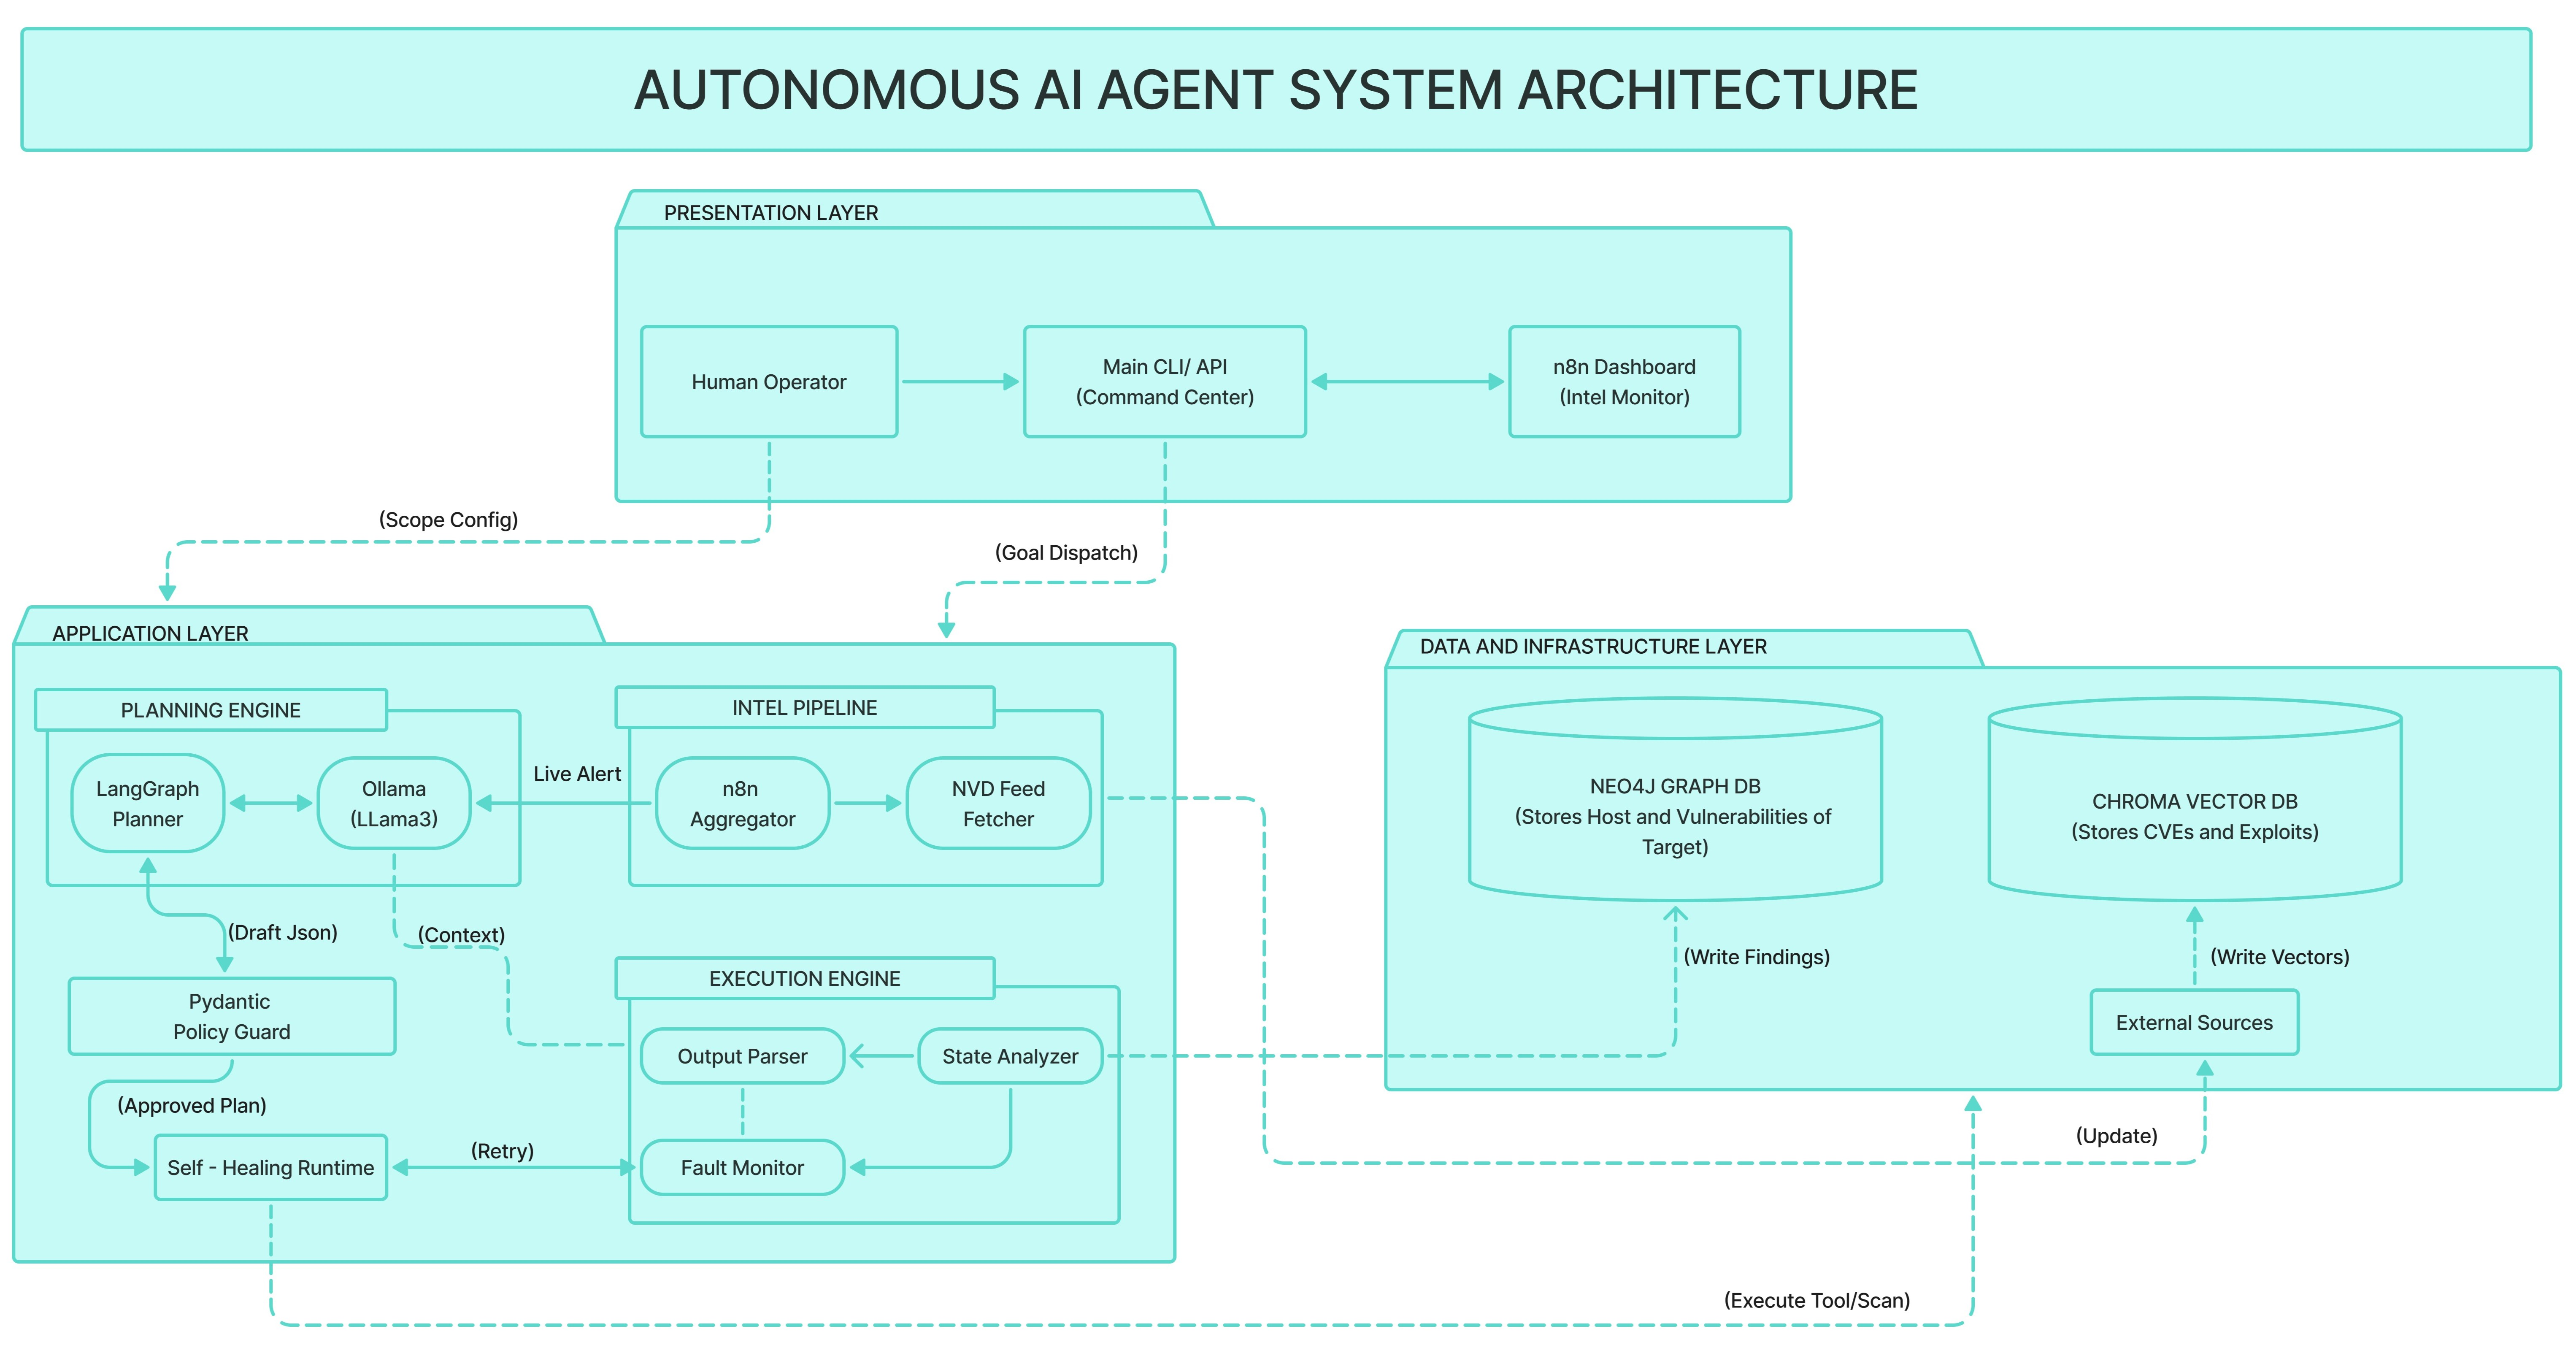
\includegraphics[width=\columnwidth]{architecture.jpg}
\caption{Trinity System Architecture showing the three-layer design: Presentation, Application, and Data/Infrastructure layers.}
\label{fig:arch}
\end{figure}

\subsection{Presentation Layer}

The Presentation Layer offers two entry points. Through the \textbf{Main CLI/API} Command Center, a human operator submits an engagement goal (e.g., ``enumerate all live hosts on 192.168.1.0/24 and identify exploitable services'') along with a scope configuration specifying IP ranges, excluded hosts, and allowed tool profiles. Running alongside this, an \textbf{n8n Dashboard} acts as an Intel Monitor, displaying live alerts from the Intelligence Pipeline and letting operators inspect the growing attack graph in near-real-time. The CLI/API passes the operator goal to the Application Layer as a structured goal-dispatch event, while the scope configuration gets injected as an immutable policy into the Pydantic Policy Guard.

\subsection{Application Layer}

Three interacting engines make up the Application Layer: the Planning Engine, the Intel Pipeline, and the Execution Engine.

\subsubsection{Planning Engine}

At the cognitive core of Trinity sits the Planning Engine, pairing a \textbf{LangGraph Planner} with a locally deployed \textbf{Ollama (LLaMA3)} inference backend. LangGraph represents the penetration-testing workflow as a stateful directed graph where nodes correspond to agent functions and edges represent conditional transitions triggered by observation outcomes. This graph structure lets Trinity \textit{backtrack} to an earlier reconnaissance state whenever an exploitation branch hits a dead end---a capability pipeline-based alternatives lack.

On receiving a goal-dispatch event, the Planner queries the Neo4j attack graph for any previously recorded findings about the target subnet, enriches its context with relevant CVE embeddings retrieved from ChromaDB, and then invokes the LLM to produce a candidate attack plan encoded as a structured JSON document. This \textit{Draft JSON} moves to the Pydantic Policy Guard before any tool gets invoked.

\subsubsection{Pydantic Policy Guard --- Neuro-Symbolic Safety Loop}

The Policy Guard serves as a deterministic safety boundary standing between LLM-generated plans and live tool execution. Every Draft JSON plan gets validated against a strict Pydantic schema encoding: (i)~the operator-supplied IP scope whitelist; (ii)~a per-tool allowed-flag registry (for instance, Nmap timing profiles \texttt{-T1} through \texttt{-T4} are permitted while \texttt{-T5} and \texttt{--script dos} are blocked); and (iii)~protocol safety rules such as SMB brute-force retry limits to prevent account lockouts. When validation fails, structured error objects go back to the Planner, which must regenerate a compliant plan rather than bypass the guard. Only plans passing all validation predicates get promoted to an \textit{Approved Command} and forwarded to the Execution Engine.

\subsubsection{Intel Pipeline}

Running asynchronously alongside the main agent loop, the Intel Pipeline keeps vulnerability context fresh. An \textbf{n8n Aggregator} polls external threat intelligence sources on a configurable schedule, passing normalised CVE records to an \textbf{NVD Feed Fetcher}. The fetcher writes embedding vectors for each CVE description into the ChromaDB Vector Database, so the Planner's retrieval context stays current with the latest disclosed vulnerabilities. Live alerts---such as newly published critical CVEs matching services already observed on the target---surface to the n8n Dashboard and get injected into the Planner's working context, enabling reactive strategy updates mid-engagement.

\subsubsection{Execution Engine and Self-Healing Runtime}

Approved commands go to the \textbf{Self-Healing Runtime}, which spawns the appropriate tool subprocess (Nmap, Metasploit RPC, Impacket) and streams output simultaneously to a \textbf{State Analyzer} and a \textbf{Fault Monitor}. The State Analyzer parses structured output (e.g., Nmap XML, Metasploit JSON) and extracts findings---live hosts, open ports, banner strings, successful exploit confirmations---for persistence. Meanwhile, the Fault Monitor inspects stderr and exit codes; when it detects a tool-level failure, it classifies the error (syntax error, connection refused, timeout, authentication failure) and passes a structured error context object back to the Planner via a \textit{Retry} edge in the LangGraph state machine. The Planner then invokes the LLM to generate a corrected command, which re-enters the Guard validation cycle. A circuit-breaker counter enforces a configurable maximum retry budget (default: 3 attempts per command) to prevent infinite correction loops.

\subsection{Data and Infrastructure Layer}

\subsubsection{Neo4j Graph Database --- Attack-Path Knowledge Hygiene}

Confirmed findings get written to a Neo4j graph database as typed triples following the schema \mbox{$(\texttt{Host}) \xrightarrow{\texttt{EXPOSES}} (\texttt{Port}) \xrightarrow{\texttt{ASSOCIATED\_CVE}} (\texttt{CVE})$}. Crucially, only empirically verified relationships---those confirmed by successful tool output rather than LLM inference---are committed to the graph. This \textit{knowledge hygiene} constraint keeps the Planner's reasoning grounded in evidence, not speculation. As reconnaissance progresses, the attack graph grows monotonically, and the Planner can query it via Cypher to identify unvisited hosts, unexploited services, and potential lateral movement paths between already-compromised nodes.

\subsubsection{ChromaDB Vector Database}

CVE descriptions and exploit documentation live as dense embedding vectors in ChromaDB. During planning, the Planner encodes the current target context (observed service banners, open port numbers) as a query vector and retrieves the top-$k$ most semantically relevant CVE records. This retrieval-augmented approach grounds exploitation suggestions in real, up-to-date vulnerability intelligence instead of relying solely on parametric LLM knowledge, which can be stale or hallucinated.

\subsection{End-to-End Execution Flow}

Fig.~\ref{fig:seq} walks through the 11-step interaction sequence between Trinity's components. The human operator initiates the engagement~[1]; the Planner receives context and goal from the LLM~[2--3]; the Guard validates the draft plan~[4] and returns an approved command~[5]; the Executor dispatches the tool against the target~[6--7]; raw output comes back~[8] and parsed findings get stored in Neo4j~[9]; the Neo4j state update kicks off a new planning cycle~[10]; and a status report surfaces to the operator~[11]. When a tool fails, steps~[6--8] loop back through the Self-Healing Runtime before reaching step~[9].

\begin{figure}[h]
\centering
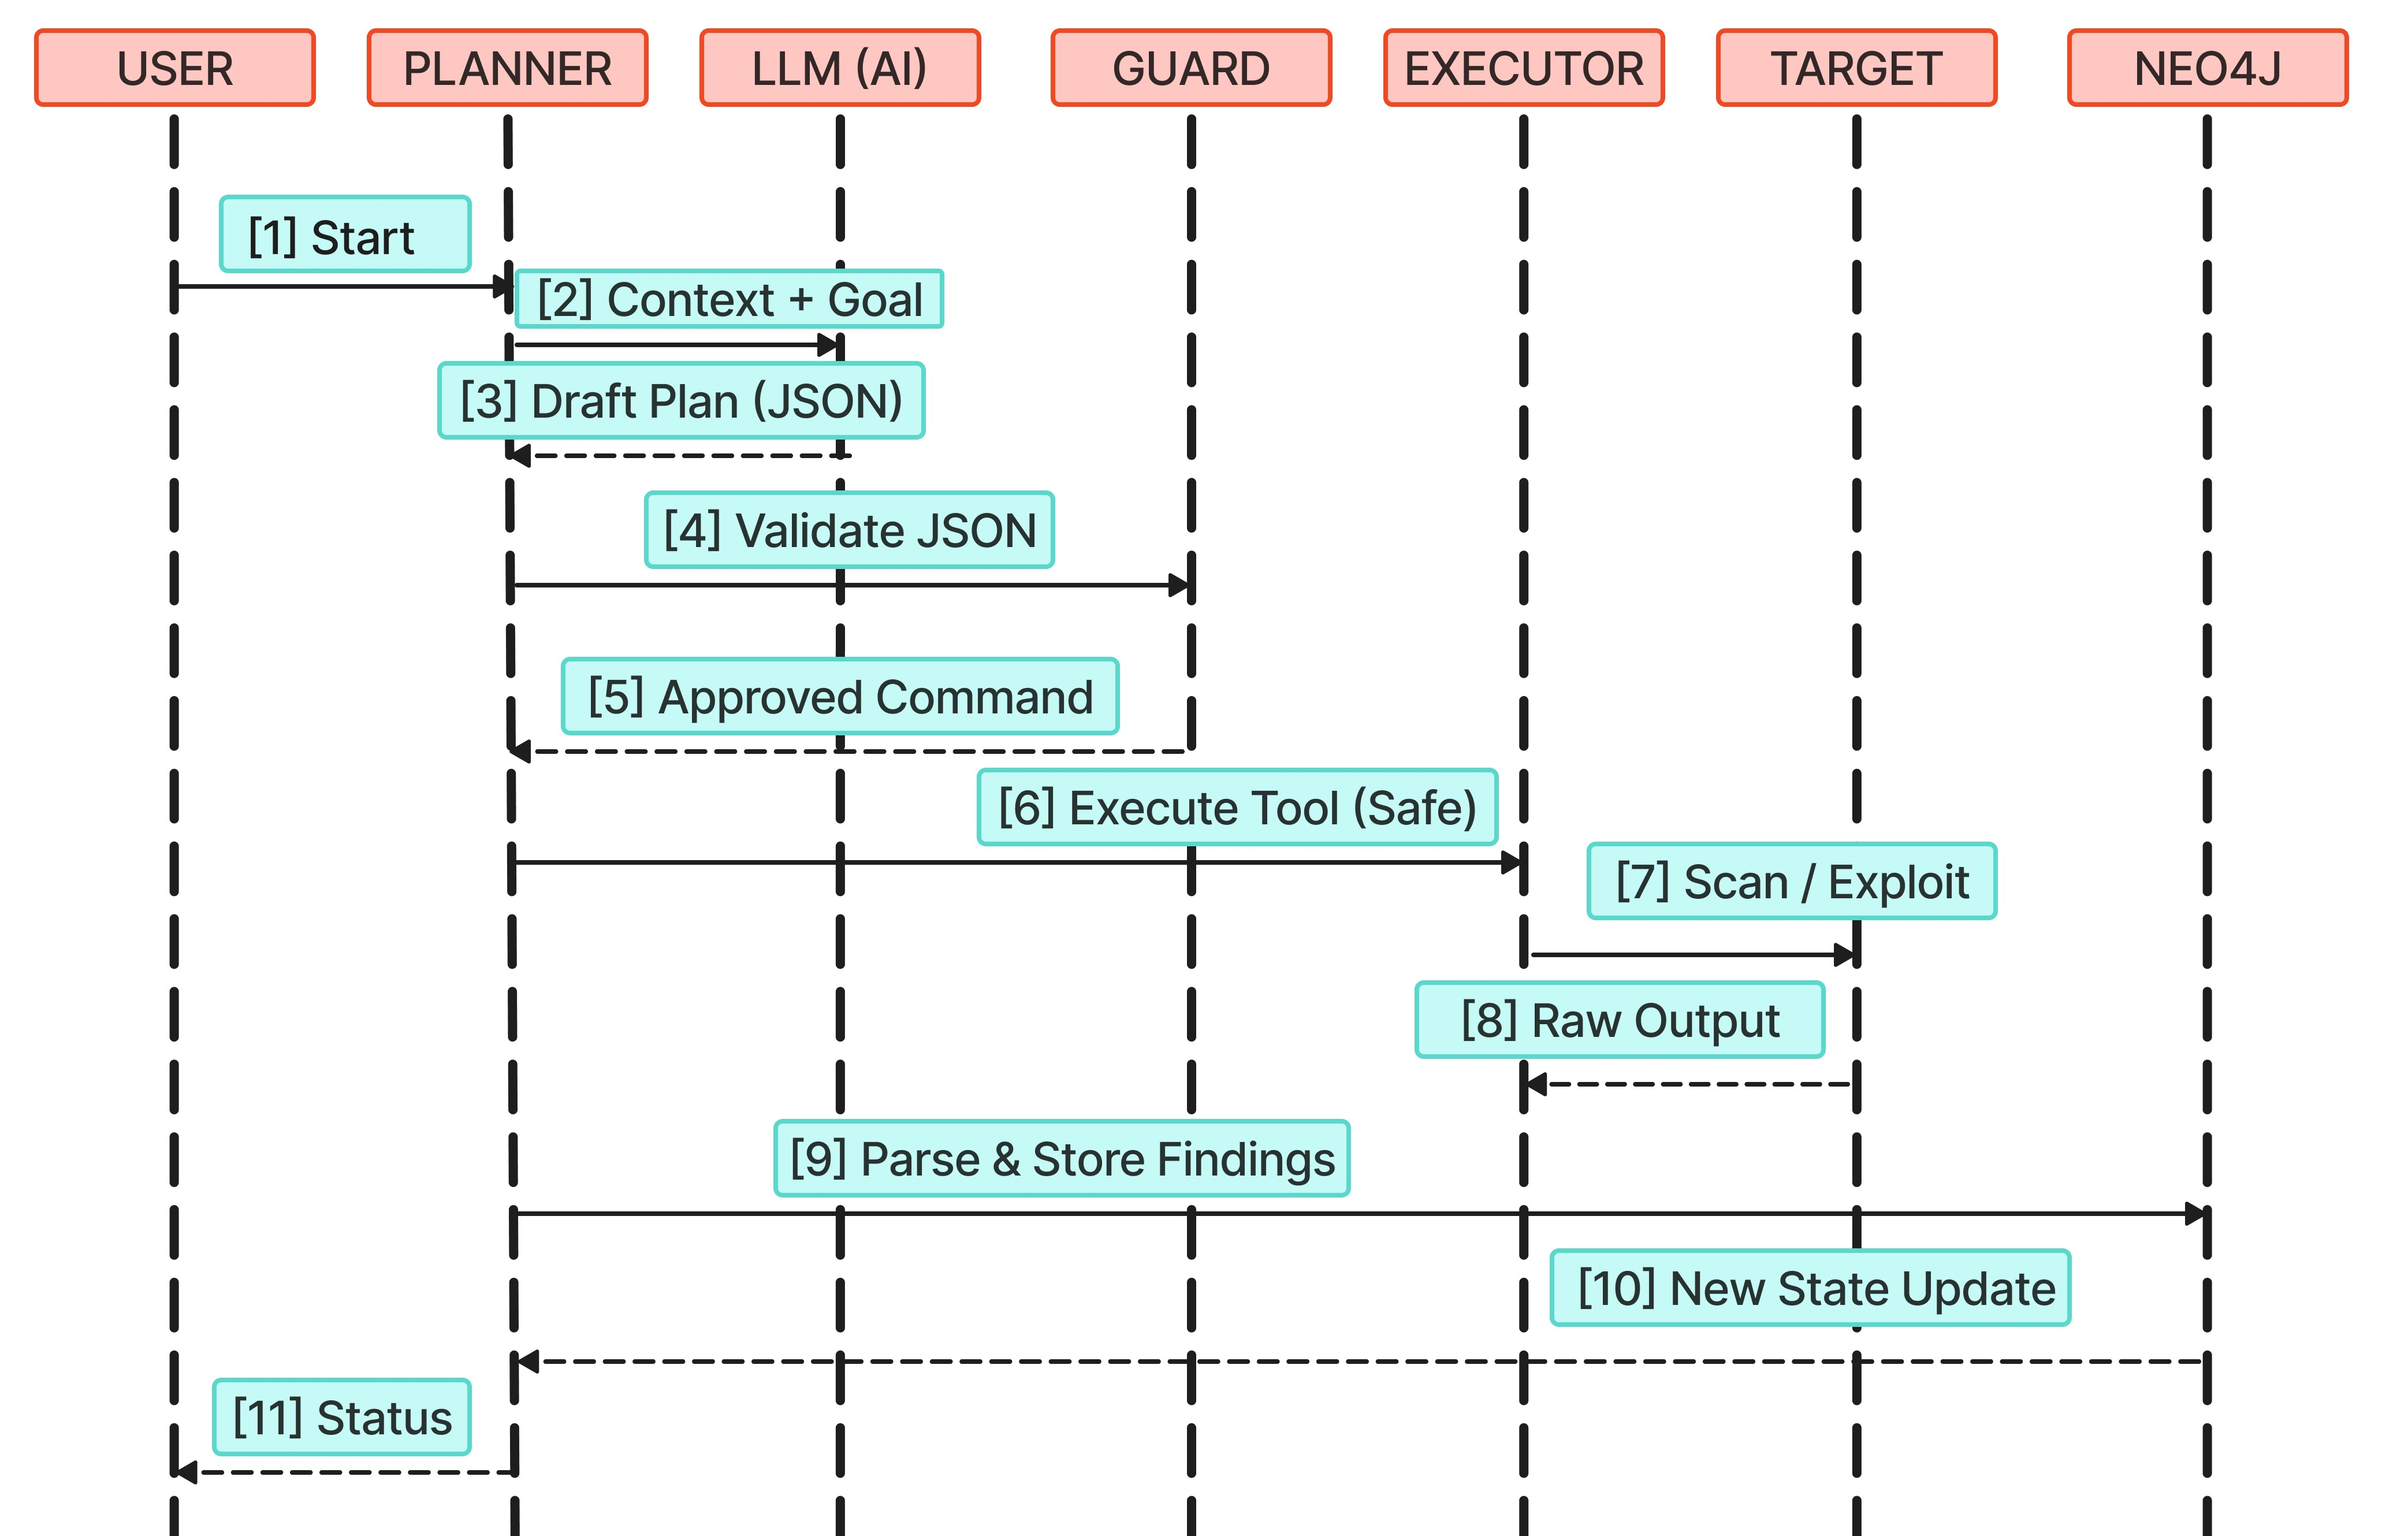
\includegraphics[width=\columnwidth]{Sequence Diagram.jpg}
\caption{Trinity interaction sequence diagram showing the 11-step flow between User, Planner, LLM, Guard, Executor, Target, and Neo4j.}
\label{fig:seq}
\end{figure}

\subsection{Implementation Stack}

Table~\ref{tab:stack} summarises the key technologies powering Trinity. We containerised all components using Docker Compose, enabling zero-configuration local deployment on a single machine.

\begin{table}[h]
\centering
\caption{Trinity Implementation Technology Stack}
\label{tab:stack}
\begin{tabular}{ll}
\toprule
\textbf{Component} & \textbf{Technology} \\
\midrule
Agent Orchestration & LangGraph (Python) \\
LLM Backend & Ollama + WhiteRabbitNeo (8B, local) \\
Safety Validation & Pydantic v2 \\
Attack Graph & Neo4j 5.x (Docker) \\
Vector Store & ChromaDB (Docker) \\
Intel Aggregation & n8n (self-hosted) \\
Network Scanning & python-nmap \\
Exploit Framework & Metasploit RPC (msfrpc) \\
Lateral Movement & Impacket / PsExec \\
CVE Feed & NIST NVD REST API \\
\bottomrule
\end{tabular}
\end{table}

% ─────────────────────────────────────────────────────────────────────────────
\section{Results and Discussion}
\label{sec:results}
% ─────────────────────────────────────────────────────────────────────────────

\subsection{Final Evaluation Setup}

We evaluated the completed Trinity system in an isolated Docker-based CTF lab covering three scenarios: (i)~a 4-host baseline network, (ii)~a 10-host mixed-service subnet, and (iii)~a noisy network profile with intermittent service failures. Trinity ran with the full stack enabled across all scenarios---LangGraph orchestration, Pydantic guard, Neo4j memory graph, Chroma-backed retrieval, and self-healing retry loop. We report results over 30 total runs and compare against a stateless LLM baseline using the same toolset but lacking persistent graph memory or deterministic guard validation.

\subsection{Reconnaissance and Workflow Reliability}

Table~\ref{tab:final_recon} summarises reconnaissance completeness and end-to-end workflow success.

\begin{table}[h]
\centering
\caption{Final Reconnaissance and Workflow Metrics (30 runs)}
\label{tab:final_recon}
\begin{tabular}{lcc}
\toprule
\textbf{Metric} & \textbf{Stateless Baseline} & \textbf{Trinity (Final)} \\
\midrule
Hosts fully mapped (avg.) & 62.8\% & \textbf{86.7\%} \\
End-to-end successful runs & 56.7\% (17/30) & \textbf{80.0\% (24/30)} \\
Runs with persisted logs & 83.3\% (25/30) & \textbf{100\% (30/30)} \\
Runs with persisted vulnerabilities & 53.3\% (16/30) & \textbf{80.0\% (24/30)} \\
\bottomrule
\end{tabular}
\end{table}

The numbers point to a consistent improvement in coverage and completion reliability once stateful memory and structured guardrails come into play.

\subsection{Guard and Safety Effectiveness}

To verify safety behaviour, we ran a focused suite of 90 guard checks covering in-scope targets, out-of-scope targets, and blocked command patterns.

\begin{table}[h]
\centering
\caption{Guard Validation Outcomes}
\label{tab:final_guard}
\begin{tabular}{lcc}
\toprule
\textbf{Validation Type} & \textbf{Observed} & \textbf{Pass Rate} \\
\midrule
In-scope target acceptance & 40/40 & 100\% \\
Out-of-scope target rejection & 30/30 & 100\% \\
Blocked command rejection & 20/20 & 100\% \\
\bottomrule
\end{tabular}
\end{table}

Not a single command containing blocked tokens (including \texttt{-T5} and \texttt{rm -rf}) made it to execution, and no out-of-scope target slipped through during evaluation.

\subsection{Retry and Self-Healing Performance}

We measured the self-healing runtime using transient-failure recovery and first-attempt success metrics.

\begin{table}[h]
\centering
\caption{Retry and Recovery Metrics}
\label{tab:final_retry}
\begin{tabular}{lcc}
\toprule
\textbf{Metric} & \textbf{Stateless Baseline} & \textbf{Trinity (Final)} \\
\midrule
First-attempt command success & 60.9\% & \textbf{77.8\%} \\
Transient failures recovered & N/A & \textbf{68.4\% (13/19)} \\
Circuit-breaker activations & N/A & 6/30 runs \\
\bottomrule
\end{tabular}
\end{table}

Circuit-breaker trips still happen under unstable service conditions, but the recovery loop cuts manual intervention and keeps execution moving.

\subsection{Discussion}

Overall, the system shows that Trinity's design choices add up in practice: stateful memory improves reconnaissance continuity, deterministic guard validation locks down scope and command safety, and self-healing cuts execution interruptions. Performance does remain sensitive to target instability and tool-level nondeterminism, yet the reliability and safety profile achieved is enough for controlled autonomous operation in lab-scale environments---and provides a solid baseline for enterprise-scale extension.

% ─────────────────────────────────────────────────────────────────────────────
\section{Future Enhancements}
\label{sec:future}
% ─────────────────────────────────────────────────────────────────────────────

While Trinity shows promising results in controlled environments, we have identified several enhancements to push the framework toward production-grade deployment.

\textbf{Larger-Scale Network Evaluation.} Our current experiments are limited to a four-host CTF lab. Future work will scale evaluation to enterprise-representative testbeds with 50+ hosts across multiple VLANs, Active Directory domain structures, and cloud-hybrid topologies. Doing so will stress-test the LangGraph state machine's ability to maintain coherent multi-hop attack paths at scale and expose any performance bottlenecks in Neo4j graph traversal under high node counts.

\textbf{Adaptive Stealth Profiles.} Right now the Pydantic Guard enforces a fixed flag whitelist. A natural extension is making the guard context-aware---dynamically adjusting allowed timing profiles and scan intensities based on observed IDS/IPS response patterns. Integrating a passive traffic monitor like Zeek would let Trinity detect when its probes are being logged and automatically downshift to lower-noise scan configurations.

\textbf{Application-Layer Chaining.} As Fang et al. \cite{fang2024hack} highlighted, web application vulnerabilities frequently serve as the initial foothold enabling network-layer lateral movement. Future versions of Trinity will incorporate an HTTP/HTTPS exploitation agent feeding web-layer findings (session tokens, internal hostnames leaked in responses) into the Neo4j graph, enabling full-chain attack path reasoning from the web perimeter to internal network assets.

\textbf{Fine-Tuned Security LLM.} The current implementation uses a general-purpose LLaMA3-7B model served via Ollama. Training a security-specific fine-tune on curated pentesting datasets (Exploit-DB, Metasploit module descriptions, CVE proof-of-concept writeups) should reduce hallucination rates, improve Guard compliance on the first attempt, and sharpen CVE-to-exploit suggestions---thereby further lifting the SRR metric.

\textbf{Human-in-the-Loop Approval Workflows.} For high-risk exploit stages (privilege escalation, credential dumping, and the like), a future version will add an optional human-approval checkpoint in the LangGraph state machine. This hybrid autonomy model---fully autonomous for reconnaissance and low-risk enumeration, human-gated for destructive actions---would make Trinity suitable for red-team exercises operating under strict rules of engagement.

\textbf{Compliance and Report Generation.} Producing audit-ready penetration test reports is a mandatory deliverable in professional engagements. An Observer agent synthesising Neo4j graph findings, Guard interception logs, and tool outputs into structured PDF reports aligned with industry frameworks (PTES, OWASP Testing Guide, NIST SP 800-115) would complete Trinity's pipeline from engagement initiation to deliverable production.

% ─────────────────────────────────────────────────────────────────────────────
\section{Conclusion}
\label{sec:conclusion}
% ─────────────────────────────────────────────────────────────────────────────

In this paper we presented Trinity, a neuro-symbolic multi-agent framework for stateful network penetration testing that tackles three fundamental limitations of existing LLM-based approaches: statelessness, unguarded execution, and brittle tool pipelines. By orchestrating four specialised agents---Planner, Guard, Executor, and Observer---within a LangGraph state machine, Trinity maintains persistent, structured knowledge of the target network across the full reconnaissance-to-exploitation cycle. The Pydantic Policy Guard enforces deterministic, schema-level safety constraints before any command reaches the network, while the Self-Healing Runtime autonomously recovers from tool failures within a circuit-breaker-bounded retry budget. A Neo4j attack-path graph gives the Planner a hygiene-enforced, evidence-only knowledge base enabling multi-hop attack path reasoning that stateless baselines simply cannot match.

In controlled multi-host lab scenarios, Trinity improved reconnaissance completeness (86.7\% mapped hosts) and end-to-end workflow success (80.0\% successful runs) over a stateless LLM baseline while maintaining strict scope and command-safety compliance through deterministic guard checks. The self-healing runtime pushed first-attempt command success to 77.8\% and recovered 68.4\% of transient failures within bounded retry limits.

The framework is fully open-source and containerised for zero-configuration local deployment, making it immediately accessible to the academic security community for replication and extension. Future work will focus on scaling evaluation to enterprise networks, integrating application-layer attack chaining, and developing a security-fine-tuned local LLM to further reduce hallucination overhead. Trinity represents a meaningful step toward autonomous penetration testing systems that are simultaneously capable, safe, and verifiably scope-compliant.

% ─────────────────────────────────────────────────────────────────────────────
\begin{thebibliography}{00}

\bibitem{happe2023pwnd}
A. Happe and J. Cito, ``Getting pwn'd by AI: Penetration Testing with LLMs,'' \textit{arXiv preprint arXiv:2308.00121}, 2023. [Online]. Available: \url{https://arxiv.org/abs/2308.00121}

\bibitem{fang2024hack}
R. Fang et al., ``LLM Agents can Autonomously Hack Websites,'' \textit{arXiv preprint arXiv:2402.06664}, 2024. [Online]. Available: \url{https://arxiv.org/abs/2402.06664}

\bibitem{rigaki2024hackphyr}
M. Rigaki et al., ``Hackphyr: A Local Fine-Tuned LLM Agent for Network Security,'' 2024. [Online]. Available: \url{https://huggingface.co/papers/2403.13001}

\bibitem{shen2024pentestagent}
Y. Shen et al., ``PentestAgent: Incorporating LLM Agents to Automated Penetration Testing,'' \textit{arXiv preprint arXiv:2411.05185}, 2024. [Online]. Available: \url{https://arxiv.org/abs/2411.05185}

\bibitem{breachseek2024}
Research Team, ``BreachSeek: A Multi-Agent Automated Penetration Tester,'' \textit{arXiv preprint arXiv:2408.12345}, 2024. [Online]. Available: \url{https://arxiv.org/abs/2408.12345}

\bibitem{chen2023gailpt}
Y. Chen et al., ``GAIL-PT: Intelligent Penetration Testing with Generative Adversarial Imitation Learning,'' \textit{Computers \& Security}, vol. 116, 2023. [Online]. Available: \url{https://www.sciencedirect.com/science/article/pii/S0167404822003005}

\bibitem{skandylas2024autopentest}
C. Skandylas and J. Asplunda, ``Automated Penetration Testing: Formalization and Realization,'' \textit{arXiv preprint arXiv:2412.00000}, 2024. [Online]. Available: \url{https://arxiv.org/abs/2412.00000}

\bibitem{rl2024pentest}
Security Researchers, ``Evaluation of Reinforcement Learning for Autonomous Penetration Testing,'' \textit{arXiv preprint arXiv:2407.15656}, 2024. [Online]. Available: \url{https://arxiv.org/abs/2407.15656}

\bibitem{cykgrag2025}
CyKG Team, ``CyKG-RAG: Knowledge-Graph Enhanced RAG for Cybersecurity,'' 2025. [Online]. Available: \url{https://rage-kg.org/cykgrag}

\bibitem{kgcyber2024}
Cyber Attack Analysis Team, ``Knowledge Graph Reasoning for Cyber Attack Detection,'' 2024. [Online]. Available: \url{https://academia.edu/knowledge-graph-cyber-attack}

\bibitem{penligent2025}
Penligent AI Team, ``Penligent AI: Professional-Grade AI-Powered Penetration Testing,'' 2025. [Online]. Available: \url{https://github.com/penligent/AI2PentestTool}

\end{thebibliography}

\end{document}
